\section{光伏功率预测实验}

\subsection{实验目的}
为了避免结课报告完全停留在文献综述层面，我配套设计了一个可在本地复现的实验，用于验证深度学习在光伏功率短时预测中的基本效果。实验目标不是追求发表级精度，而是通过统一的数据流程和对比框架，直观展示深度学习模型与简单基线模型之间的差异，从而增强报告的实践性和可信度。实验代码开源在我的 GitHub 仓库,如图~\ref{fig:experiment-code}：\url{https://github.com/glance02/SmartEnergyPVForecasting}。

\begin{figure}[H]
    \centering
    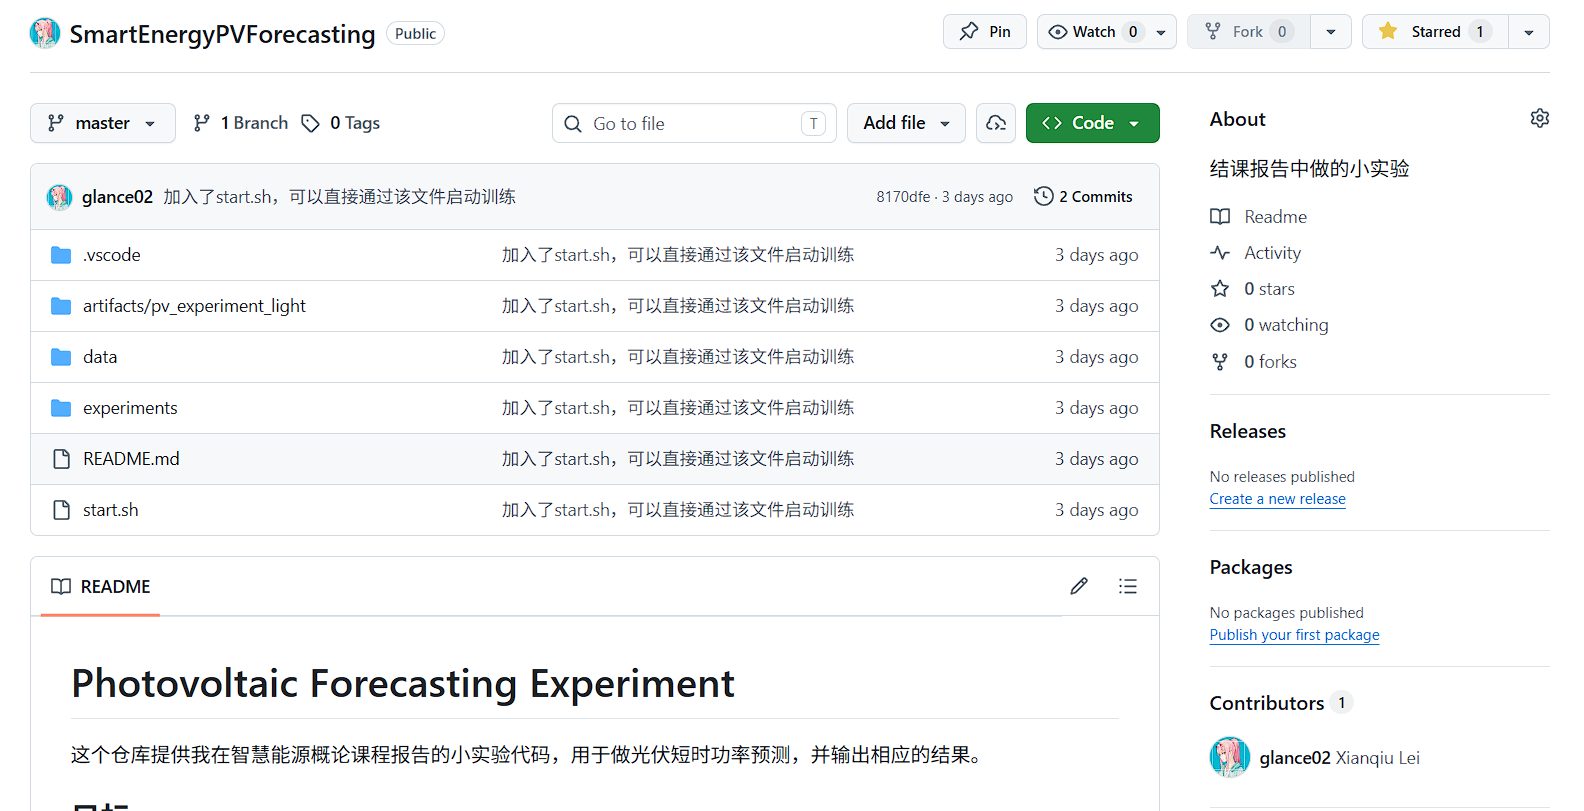
\includegraphics[width=0.45\textwidth]{Img/experiment.png}
    \captionof{figure}{开源代码界面\\Fig. 2 Source code interface}
    \label{fig:experiment-code}
\end{figure}

该实验采用 Zenodo 平台公开数据集“LIGHT dataset sample for solar smart home pilot - 201801”中的一个真实光伏站点样本，选取 \texttt{ID00002} 作为研究对象。原始数据为 1 分钟粒度的功率序列，相邻时刻之间连续性很强，因此实验将其重采样为 45 分钟粒度，以更清晰地呈现光伏功率在昼夜转换、白天爬升、峰值波动和回落过程中的变化特征，并保留单站点功率序列作为核心输入。配套实验脚本位于 \texttt{experiments}中，\texttt{experiments/main.py}用于完成训练、评估并保存模型权重和实验配置，\texttt{experiments/vis.py} 基于这些结果生成预测曲线图和简短报告摘要。更具体的解释可以查看该仓库的 README 文件以及具体代码。

\subsection{实验方案}
实验设置三类模型。第一类是 Persistence 基线，即“未来时刻功率约等于当前时刻功率”，这是时序预测中非常常见且很有参考价值的强基线。第二类是 MLP 模型，它把历史窗口展开后输入前馈神经网络，用来表示“没有显式时序记忆结构的神经网络”能达到什么水平。第三类是单层 LSTM 模型，用来体现深度学习对序列依赖关系的建模优势。LSTM也是老师在课程中介绍过、我在课堂展示中也进一步讲解过的经典时序模型。

本实验采用以下配置。首先，将原始 1 分钟数据重采样为 45 分钟数据；其次，加入基于时间戳构造的周期性时间特征，包括昼夜周期和周内周期；再次，使用过去 12 个时间步，也就是过去 9 小时的数据，预测未来 2 个时间步，也就是未来 90 分钟的光伏功率。数据经过时间排序后，保留完整的昼夜功率变化，不使用夜间过滤，并按 70\%/15\%/15\% 切分为训练集、验证集和测试集。训练阶段采用验证集 RMSE 做早停，并对重采样粒度、预测步长、窗口长度、隐藏层宽度和 batch size 做了简单调参，最终选择 \texttt{hidden\_size=128}、\texttt{batch\_size=32} 这一组参数。这样的设置既保留了全天连续功率曲线，也使数据同时呈现夜间低值、白天爬升、峰值波动和回落等不同阶段的特征，从而更贴近真实光伏功率序列在较长时间尺度下的时序结构。

\subsection{实验结果}
基于上述真实数据和配置，我最终保留的最佳实验结果表~\ref{tab:experiment-results}。从表~\ref{tab:experiment-results} 可以看出，在“45 分钟重采样 + 时间特征 + 90 分钟 ahead 预测 + 保留完整昼夜序列”的设置下，LSTM 在 MAE、RMSE 和 MAPE 三项指标上都表现最好。其中，LSTM 的 RMSE 为 0.3630，较 Persistence 下降约 13.28\%，较 MLP 下降约 17.95\%。这说明即便不使用夜间过滤，只要适当拉长时间粒度和预测步长，LSTM 对较长时序依赖和非线性变化的建模优势依然能够体现出来。

\begin{center}
\captionof{table}{实验结果\\Table 3 Experimental results on real data}
\vspace{3pt}
{\fontsize{9pt}{14pt}\selectfont
\setlength{\tabcolsep}{4pt}
\begin{tabular}{@{}lccc@{}}
\toprule
Model & MAE & RMSE & MAPE(\%) \\
\midrule
LSTM & 0.1951 & 0.3630 & 56.49 \\
Persistence & 0.2306 & 0.4186 & 139.77 \\
MLP & 0.2538 & 0.4424 & 64.61 \\
\bottomrule
\end{tabular}}
\label{tab:experiment-results}
\end{center}

需要说明的是，Persistence 的 MAPE 数值依然偏大，主要是因为光伏功率在夜间、日出和日落等低功率时段接近零，百分比误差容易被放大。因此，在解释结果时应更关注 RMSE 和 MAE 这类对工程应用更稳定的指标。综合来看，本实验支持这样一个判断：在完整昼夜预测设定下，深度学习模型能否优于强基线，并不只取决于是否保留夜间样本，还与重采样粒度、预测步长和历史窗口长度等实验口径密切相关。当前这组 45 分钟重采样、90 分钟 ahead 的设置下，LSTM 在保持完整时间轴的前提下取得最优结果。

\begin{center}

\includegraphics[width=\columnwidth]{img/fig2_prediction_curve.png}
\captionof{figure}{测试集整段时间上的真实值与各模型预测曲线\\Fig. 3 Actual and predicted curves on the test set}
\label{fig:prediction-curve}
\end{center}

\subsection{意义与启示}
本实验的意义在于，它在真实光伏数据上给出了一个结构清晰、过程完整且结果可解释的验证案例。通过与 Persistence 和 MLP 的对比，可以更具体地说明深度学习在光伏功率预测中的优势主要体现在对时序依赖关系和非线性变化的建模上，而这种优势并不是无条件成立的，仍然受到数据质量、特征设计、时间粒度和预测步长等因素的共同影响。因而，这一实验不仅补充了前文的文献分析，也进一步说明了深度学习在智慧能源场景中的有效性与适用边界。
